\documentclass{../../slides-style}

\slidetitle{Лекция 7: Структурные и порождающие шаблоны}{13.10.2022}

\begin{document}

    \begin{frame}[plain]
        \titlepage
    \end{frame}

    \section{Паттерн ``Мост''}

    \begin{frame}
        \frametitle{Паттерн ``Мост'' (Bridge)}
        Отделяет абстракцию от реализации

        Пример:
        \begin{itemize}
            \item Есть система, интерпретирующая программы для роботов
            \item Есть класс \textit{Sensor}, от которого наследуются \textit{SonarSensor}, \textit{LightSensor}, ...
            \item Связь с роботом может выполняться по USB или Bluetooth, а может быть, программа и вовсе исполняется на симуляторе
            \item Интерпретатор хочет работать с сенсорами, не заморачиваясь реализацией механизма связи
            \item Рабоче-крестьянская реализация --- \textit{USBLightSensor}, \textit{BluetoothLightSensor}, \textit{USBSonarSensor}, \textit{BluetoothSonarSensor}, ...
            \item Число классов --- произведение количества сенсоров и типов связи
        \end{itemize}
    \end{frame}

    \begin{frame}
        \frametitle{``Мост'', пример}
        \begin{center}
            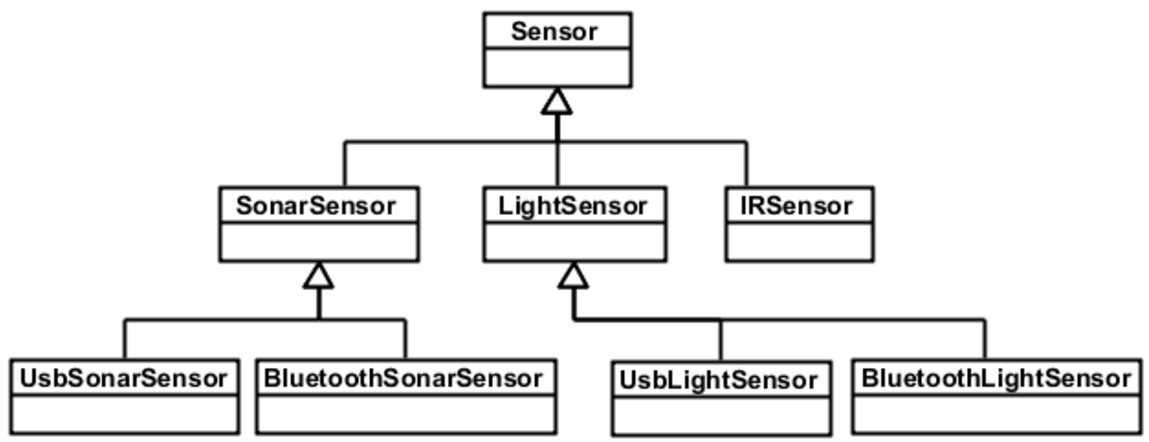
\includegraphics[width=0.7\textwidth]{noBridge.png}
            \Huge{$$\downarrow$$}
            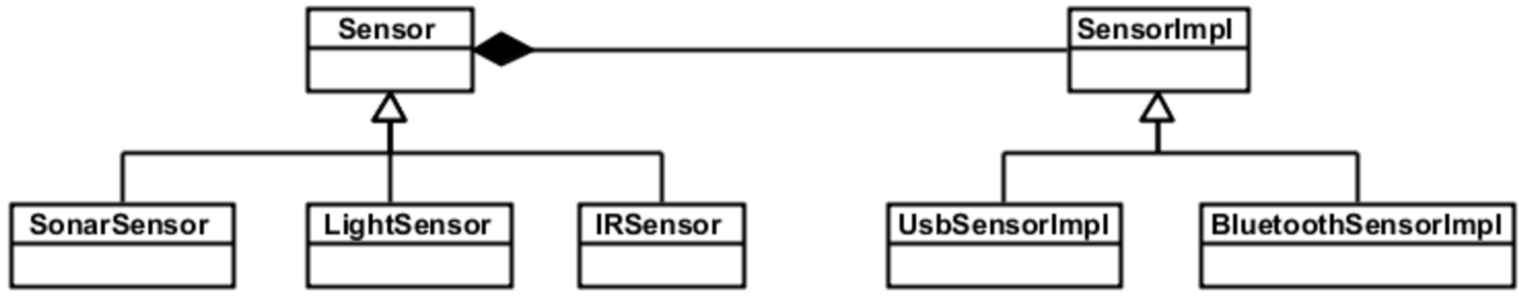
\includegraphics[width=0.7\textwidth]{bridge.png}
        \end{center}
    \end{frame}

    \begin{frame}
        \frametitle{``Мост'', общая схема}
        \begin{center}
            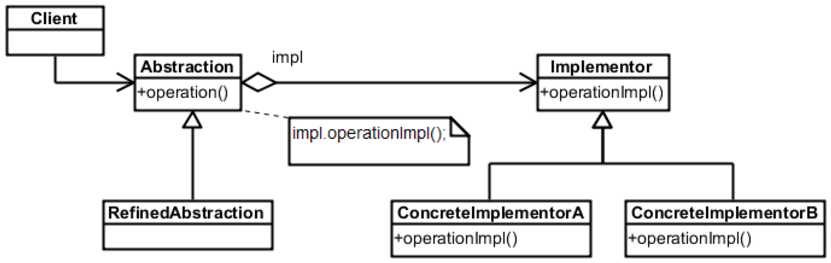
\includegraphics[width=0.7\textwidth]{bridgeGeneral.png}
        \end{center}
        \begin{itemize}
            \item \textit{Abstraction} --- определяет интерфейс абстракции, хранит ссылку на реализацию
            \item \textit{RefinedAbstraction} --- расширяет интерфейс абстракции, делает полезную работу, используя реализацию
            \item \textit{Implementor} --- определяет интерфейс реализации, в котором абстракции предоставляются низкоуровневые операции
            \item \textit{ConcreteImplementor} --- предоставляет конкретную реализацию Implementor
        \end{itemize}
    \end{frame}

    \begin{frame}
        \frametitle{Когда применять}
        \begin{itemize}
            \item Когда хочется разделить абстракцию и реализацию, например, когда реализацию можно выбирать во время компиляции или во время выполнения
            \begin{itemize}
                \item ``Стратегия'', ``Прокси''
            \end{itemize}
            \item Когда абстракция и реализация должны расширяться новыми подклассами
            \item Когда хочется разделить одну реализацию между несколькими объектами
            \begin{itemize}
                \item Как copy-on-write в строках
            \end{itemize}
        \end{itemize}
    \end{frame}

    \begin{frame}
        \frametitle{Тонкости реализации}
        Создание правильного Implementor-а
        \begin{itemize}
            \item Самой абстракцией в конструкторе, в зависимости от переданных параметров
            \begin{itemize}
                \item Как вариант --- выбор реализации по умолчанию и замена её по ходу работы
            \end{itemize}
            \item Принимать реализацию извне (как параметр конструктора, или, реже, как значение в сеттер)
            \item Фабрика/фабричный метод
            \begin{itemize}
                \item Позволяет спрятать платформозависимые реализации, чтобы не зависеть от них всех при сборке
            \end{itemize}
        \end{itemize}
    \end{frame}

    \begin{frame}
        \frametitle{Pointer To Implementation (PImpl)}
        Вырожденный мост для C++, когда ``абстракция'' имеет ровно одну реализацию, часто полностью дублирующую её интерфейс

        Зачем: чтобы клиенты класса не зависели при сборке от его реализации

        \begin{itemize}
            \item Позитивно сказывается на времени компиляции программ на C++
            \item Позволяет менять реализацию независимо
        \end{itemize}

        Как: предварительное объявление класса-реализации, полное определение --- в .cpp-файле вместе с методами абстракции

        \begin{center}
            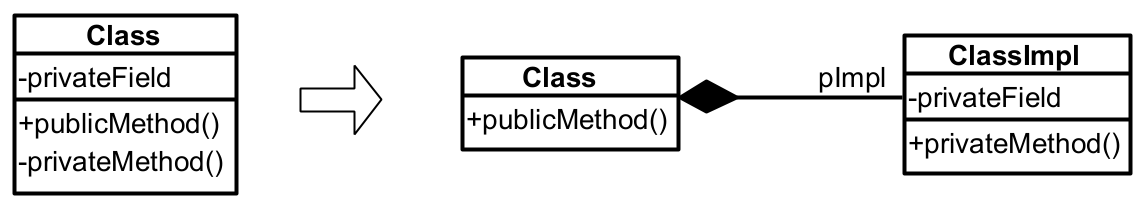
\includegraphics[width=0.6\textwidth]{pImpl.png}
        \end{center}

        Часто используется в реализации библиотек (например, Qt)
    \end{frame}

    \section{Паттерн ``Фабричный метод''}

    \begin{frame}
        \frametitle{``Фабричный метод'' мотивация}
        \framesubtitle{Игра-стратегия}
        \begin{columns}
            \begin{column}{0.5\textwidth}
                \begin{itemize}
                    \item Воины
                    \begin{itemize}
                        \item Мечники
                        \item Конница
                        \item Лучники
                    \end{itemize}
                    \item Общее поведение
                    \item Общие характеристики
                \end{itemize}
            \end{column}
            \begin{column}{0.5\textwidth}
                \begin{center}
                    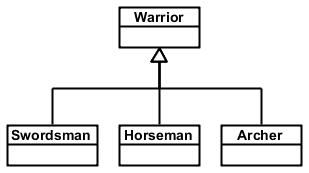
\includegraphics[width=0.8\textwidth]{warriors.png}
                \end{center}
            \end{column}
        \end{columns}
    \end{frame}

    \begin{frame}[fragile]
        \frametitle{Виртуальный конструктор}
        \begin{columns}
            \begin{column}{0.6\textwidth}
                \begin{footnotesize}
                    \begin{minted}{c++}
enum WarriorId { SwordsmanId, ArcherId, HorsemanId };

class Warrior
{
public:  
    Warrior(WarriorId id)
    {
        if (id == SwordsmanId) p = new Swordsman;
        else if (id == ArcherId) p = new Archer;
        else if (id == HorsemanId) p = new Horseman;
        else assert(false);
    }
    virtual void info() { p->info(); }
    virtual ~Warrior() { delete p;  p = 0; }
private:
    Warrior* p;
};
                    \end{minted}
                \end{footnotesize}
            \end{column}
            \begin{column}{0.4\textwidth}
                \begin{center}
                    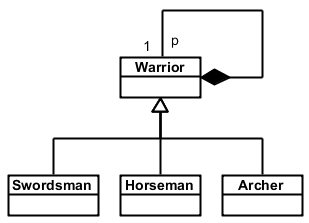
\includegraphics[width=0.95\textwidth]{warriorVirtualCtor.png}
                \end{center}
            \end{column}
        \end{columns}
    \end{frame}

    \begin{frame}
        \frametitle{Фабричный метод}
        \begin{columns}
            \begin{column}{0.5\textwidth}
                \begin{itemize}
                    \item Базовый класс знает про остальные
                    \item switch в createWarrior()
                \end{itemize}
            \end{column}
            \begin{column}{0.5\textwidth}
                \begin{center}
                    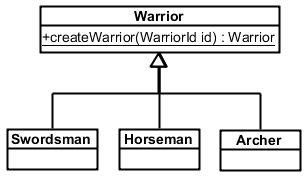
\includegraphics[width=0.8\textwidth]{warriorFactoryMethod.png}
                \end{center}
            \end{column}
        \end{columns}
    \end{frame}

    \begin{frame}
        \frametitle{Паттерн ``Factory Method''}
        \framesubtitle{Factory Method}
        \begin{center}
            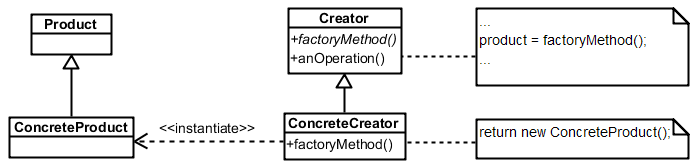
\includegraphics[width=0.8\textwidth]{factoryMethod.png}
        \end{center}
        \begin{itemize}
            \item Применимость:
            \begin{itemize}
                \item классу заранее неизвестно, объекты каких классов ему нужно создавать
                \item объекты, которые создает класс, специфицируются подклассами
                \item класс делегирует свои обязанности одному из нескольких вспомогательных подклассов
            \end{itemize}
        \end{itemize}
    \end{frame}

    \begin{frame}
        \frametitle{Пример, текстовый редактор}
        \begin{center}
            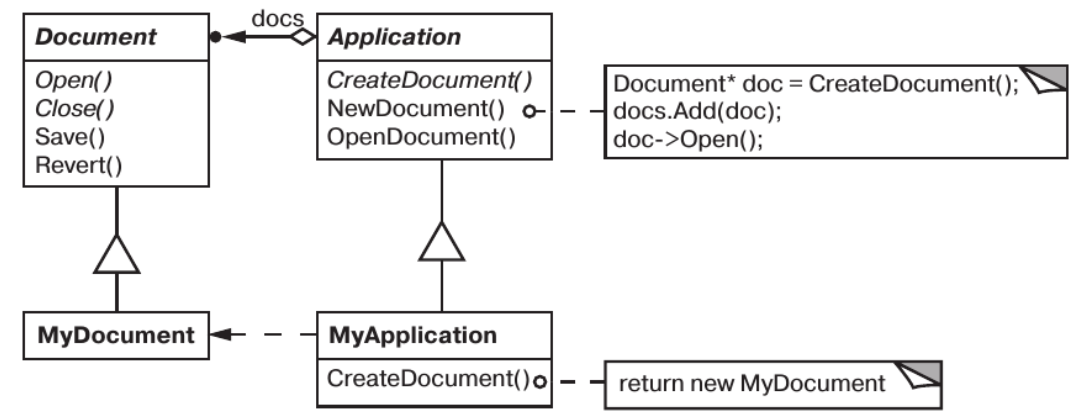
\includegraphics[width=0.9\textwidth]{factoryMethodForTextEditor.png}
        \end{center}
    \end{frame}

    \begin{frame}
        \frametitle{``Фабричный метод'', детали реализации}
        \begin{center}
            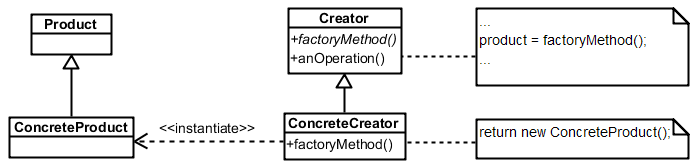
\includegraphics[width=0.6\textwidth]{factoryMethod.png}
        \end{center}
        \begin{itemize}
            \item Абстрактный Creator или реализация по умолчанию
            \begin{itemize}
                \item Второй вариант может быть полезен для расширяемости
            \end{itemize}
            \item Параметризованные фабричные методы
            \item Если язык поддерживает инстанциацию по прототипу (JavaScript, Smalltalk), можно хранить порождаемый объект
            \item Creator не может вызывать фабричный метод в конструкторе
            \item Можно сделать шаблонный Creator
            \item Можно использовать лямбда-функции
        \end{itemize}
    \end{frame}

    \section{Паттерн ``Абстрактная фабрика''}

    \begin{frame}
        \frametitle{``Абстрактная фабрика'', мотивация}
        \begin{itemize}
            \item Хотим поддержать разные стили UI
            \begin{itemize}
                \item Гибкая поддержка в архитектуре
                \item Удобное добавление новых стилей
            \end{itemize}
        \end{itemize}
        \begin{center}
            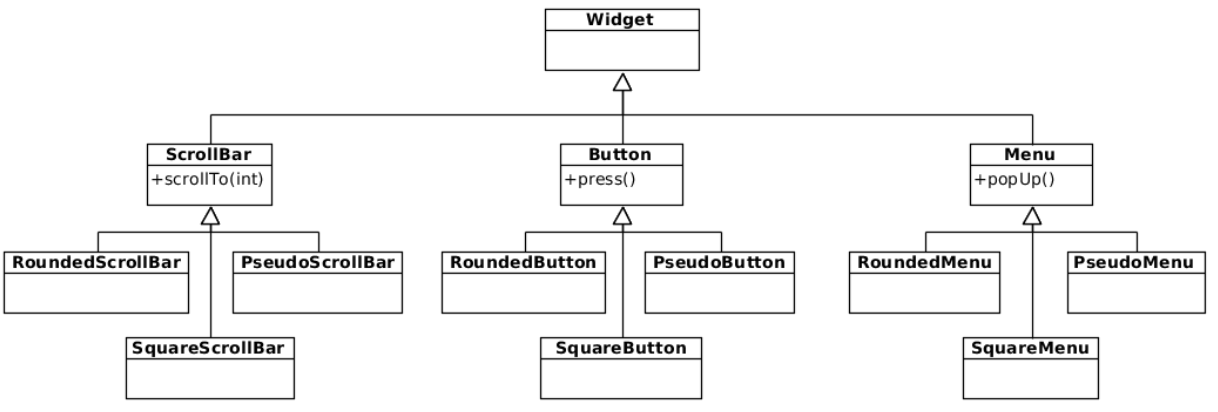
\includegraphics[width=0.95\textwidth]{widgets.png}
        \end{center}
    \end{frame}

    \begin{frame}
        \frametitle{Создание виджетов}
        \mintinline{c++}|ScrollBar* bar = new RoundedScrollBar;|
        
        \vspace{2mm}
        
        vs
        
        \vspace{2mm}
        
        \mintinline{c++}|ScrollBar* bar = guiFactory->createScrollBar();|
    \end{frame}

    \begin{frame}
        \frametitle{Фабрика виджетов}
        \begin{center}
            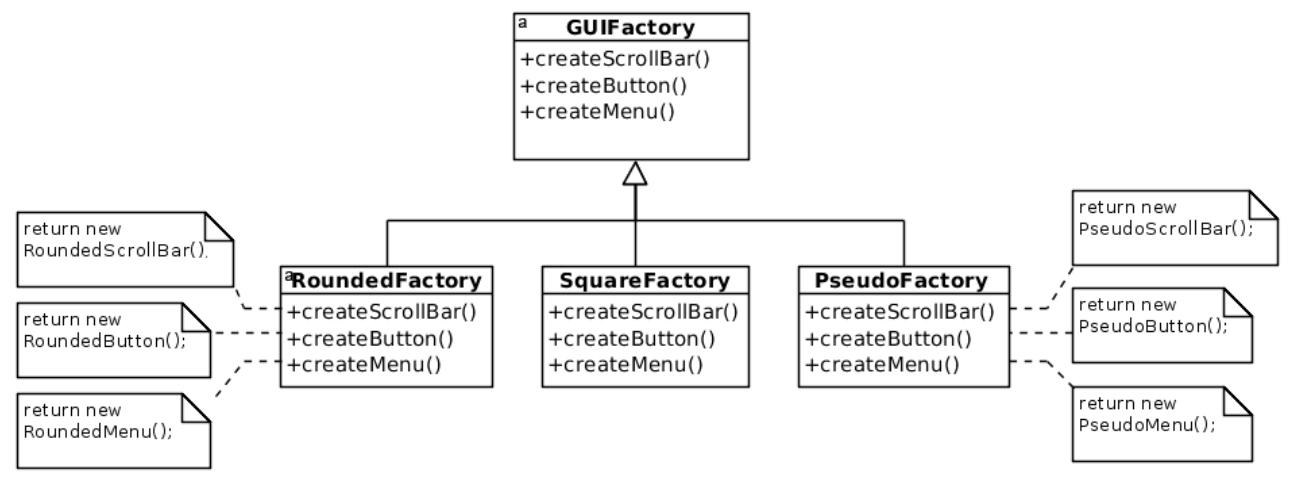
\includegraphics[width=0.95\textwidth]{widgetFactory.png}
        \end{center}
    \end{frame}

    \begin{frame}
        \frametitle{Паттерн ``Абстрактная фабрика''}
        \framesubtitle{Abstract Factory}
        \begin{columns}
            \begin{column}{0.4\textwidth}
                \begin{itemize}
                    \item Изолирует конкретные классы
                    \item Упрощает замену семейств продуктов
                    \item Гарантирует сочетаемость продуктов
                    \item Поддержать новый вид продуктов непросто
                \end{itemize}
            \end{column}
            \begin{column}{0.6\textwidth}
                \begin{center}
                    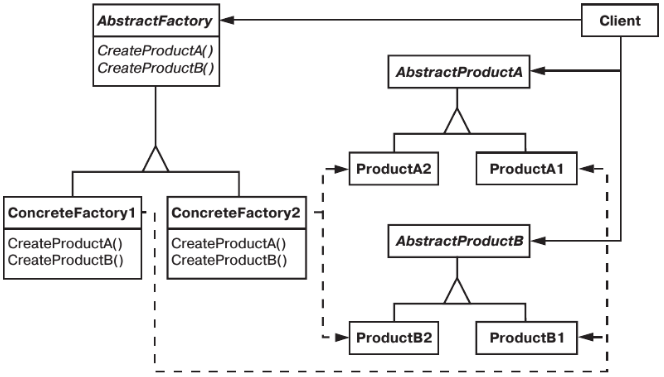
\includegraphics[width=0.95\textwidth]{abstractFactory.png}
                \end{center}
            \end{column}
        \end{columns}
    \end{frame}

    \begin{frame}
        \frametitle{``Абстрактная фабрика'', применимость}
        \begin{itemize}
            \item Система не должна зависеть от того, как создаются, компонуются и представляются входящие в неё объекты
            \item Система должна конфигурироваться одним из семейств составляющих её объектов
            \item Взаимосвязанные объекты должны использоваться вместе
            \item Хотите предоставить библиотеку объектов, раскрывая только их интерфейсы, но не реализацию
        \end{itemize}
    \end{frame}

    \begin{frame}
        \frametitle{``Абстрактная фабрика'', детали реализации}
        \begin{columns}
            \begin{column}{0.5\textwidth}
                \begin{itemize}
                    \item Хорошо комбинируются с паттерном ``Одиночка''
                    \item Если семейств продуктов много, то фабрика может инициализироваться \textit{прототипами}, тогда не надо создавать сотню подклассов
                \end{itemize}
            \end{column}
            \begin{column}{0.5\textwidth}
                \begin{center}
                    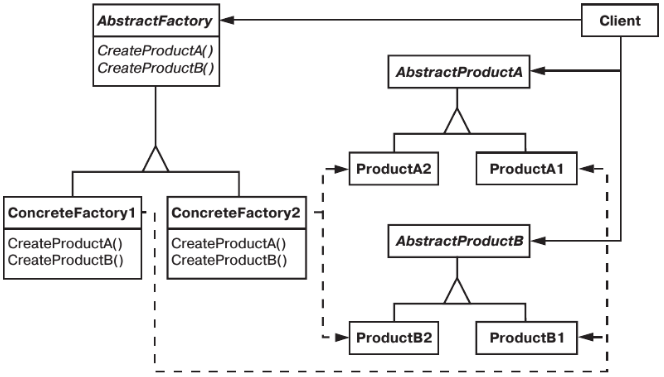
\includegraphics[width=\textwidth]{abstractFactory.png}
                \end{center}
            \end{column}
        \end{columns}
        \begin{itemize}
            \item Прототип на самом деле может быть классом (например, Class в Java)
            \item Если виды объектов часто меняются, может помочь параметризация метода создания
            \begin{itemize}
                \item Может пострадать типобезопасность
            \end{itemize}
        \end{itemize}
    \end{frame}

    \section{Паттерн ``Одиночка''}

    \begin{frame}
        \frametitle{Паттерн ``Одиночка''}
        \framesubtitle{Singleton}
        \begin{columns}
            \begin{column}{0.6\textwidth}
                \begin{itemize}
                    \item Гарантирует, что у класса есть только один экземпляр
                    \item Предоставляет глобальный доступ к этому экземпляру
                    \item Позволяет использовать подклассы без модификации клиентского кода
                \end{itemize}
            \end{column}
            \begin{column}{0.4\textwidth}
                \begin{center}
                    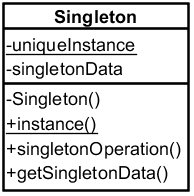
\includegraphics[width=0.6\textwidth]{singleton.png}
                \end{center}
            \end{column}
        \end{columns}
    \end{frame}

    \begin{frame}[fragile]
        \frametitle{``Одиночка'', наивная реализация}
        \begin{minted}{java}
public class Singleton {
    private static Singleton instance;

    private Singleton () {}

    public static Singleton getInstance() {
        if (instance == null) {
            instance = new Singleton();
        }
        return instance;
    }
}
        \end{minted}
    \end{frame}

    \begin{frame}[fragile]
        \frametitle{``Одиночка'', простая многопоточная реализация}
        \begin{minted}{java}
public class Singleton {
    private static Singleton instance = new Singleton();

    private Singleton () {}

    public static Singleton getInstance() {
        return instance;
    }
}
        \end{minted}
    \end{frame}

    \begin{frame}[fragile]
        \frametitle{``Одиночка'', плохая многопоточная реализация}
        \begin{minted}{java}
public class Singleton {
    private static Singleton instance;

    public static synchronized Singleton getInstance() {
        if (instance == null) {
            instance = new Singleton();
        }
        return instance;
    }
}
        \end{minted}
    \end{frame}

    \begin{frame}[fragile]
        \frametitle{Double-checked locking}
        \framesubtitle{Более-менее хорошая многопоточная реализация}
        \begin{small}
            \begin{minted}{java}
public class Singleton {
    private static volatile Singleton instance;

    public static Singleton getInstance() {
        Singleton localInstance = instance;
        if (localInstance == null) {
            synchronized (Singleton.class) {
                localInstance = instance;
                if (localInstance == null) {
                    instance = localInstance = new Singleton();
                }
            }
        }
        return localInstance;
    }
}
            \end{minted}
        \end{small}
    \end{frame}

    \begin{frame}
        \frametitle{``Multiton''}
        \begin{columns}
            \begin{column}{0.6\textwidth}
                \begin{itemize}
                    \item Реестр одиночек, обеспечивает уникальность объекта по ключу
                    \begin{itemize}
                        \item Сам создаёт объекты
                        \item Не даёт возможности зарегистрировать объект извне
                    \end{itemize}
                \end{itemize}
            \end{column}
            \begin{column}{0.4\textwidth}
                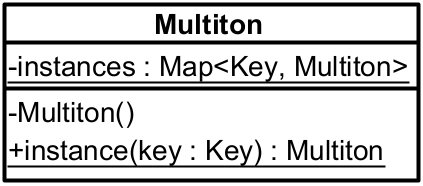
\includegraphics[width=\textwidth]{multiton.png}
            \end{column}
        \end{columns}
    \end{frame}

    \begin{frame}
        \frametitle{``Одиночка'', критика}
        \begin{itemize}
            \item Добавляет неочевидные зависимости по данным
            \begin{itemize}
                \item По сути, хитрая глобальная переменная
            \end{itemize}
            \item Усложняет тестирование
            \item Нарушает принцип единственности ответственности
            \item Сложно рефакторить, если потребуется несколько экземпляров
        \end{itemize}
    \end{frame}

    \section{Паттерн ``Ленивая инициализация''}

    \begin{frame}
        \frametitle{Паттерн ``Ленивая инициализация''}
        \begin{itemize}
            \item Некоторое упрощение одиночки
            \item Действие не выполняется до тех пор, пока не нужен его результат
            \item Используется повсеместно, для ускорения запуска и экономии на редких вычислениях
            \begin{itemize}
                \item Just-In-Time-компиляция
                \item Ленивые структуры данных (списки в Haskell, seq в F\#)
                \item Ленивые вычисления (Haskell, Lazy<T> в .NET)
                \item ...
            \end{itemize}
            \item Имеет те же проблемы с многопоточностью, что и одиночка
        \end{itemize}
    \end{frame}

    \section{Паттерн ``Пул объектов''}

    \begin{frame}
        \frametitle{Паттерн ``Пул объектов'', мотивация}
        \framesubtitle{Потоки в .NET}
        \begin{itemize}
            \item Класс Thread, конструктор создаёт поток и запускает в нём переданную операцию
            \item Поток уничтожается, когда операция завершилась
            \item Создание и остановка потоков --- долгие операции
            \item Каждый поток требует системных ресурсов
            \item Нет смысла иметь больше потоков, чем ядер процессора
        \end{itemize}
    \end{frame}

    \begin{frame}
        \frametitle{Паттерн ``Пул объектов''}
        \framesubtitle{Решение: пул потоков в .NET}
        \begin{itemize}
            \item Класс ThreadPool, синглтон
            \item Создаёт заранее N потоков, которые никогда не заканчиваются и ждут задач
            \item QueueUserWorkItem принимает задачу на исполнение
            \begin{itemize}
                \item Например, 
                \begin{footnotesize}
                    \mintinline{csharp}|ThreadPool.QueueUserWorkItem(() => Console.WriteLine("Goodbye, world!"))|
                \end{footnotesize}
            \end{itemize}
            \item Если есть свободный поток, он начинает исполнять задачу
            \item Если свободных потоков нет, а задач много, создаётся новый поток
            \item Лишние потоки удаляются, если задач нет и число потоков больше N
        \end{itemize}
    \end{frame}

    \begin{frame}
        \frametitle{Паттерн ``Пул объектов''}
        \begin{itemize}
            \item Применяется, когда объекты создавать сложно, но каждый объект нужен лишь ненадолго
            \item Желательно, чтобы на поддержание объектов в пуле не требовалось много ресурсов, либо объектов в пуле было мало
            \begin{itemize}
                \item Например, создать 50000 сетевых соединений ``заранее'' может быть плохой идеей
            \end{itemize}
            \item Следует применять с осторожностью в языках со сборкой мусора --- пул держит ссылки на объекты
            \begin{itemize}
                \item К тому же, в таких языках new отрабатывает мгновенно
            \end{itemize}
            \item Следует помнить про многопоточность
            \begin{itemize}
                \item Как правило, методы пула требуют синхронизации
            \end{itemize}
        \end{itemize}
    \end{frame}

    \section{Паттерн ``Прототип''}

    \begin{frame}
        \frametitle{``Прототип'', мотивация}
        \begin{center}
            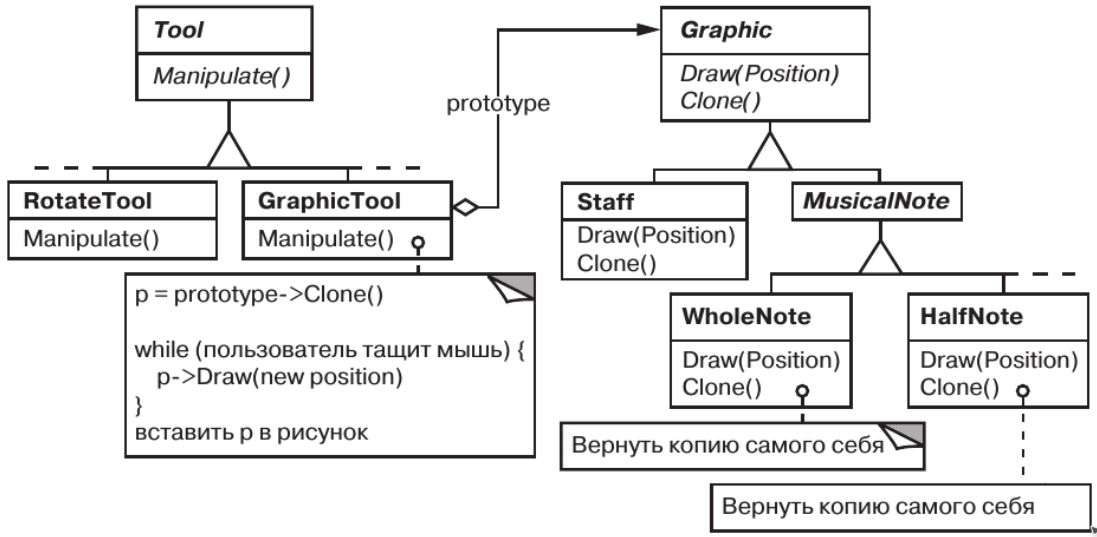
\includegraphics[width=0.9\textwidth]{musicalEditor.png}
        \end{center}
    \end{frame}

    \begin{frame}
        \frametitle{Паттерн ``Прототип''}
        \framesubtitle{Prototype}
        \begin{center}
            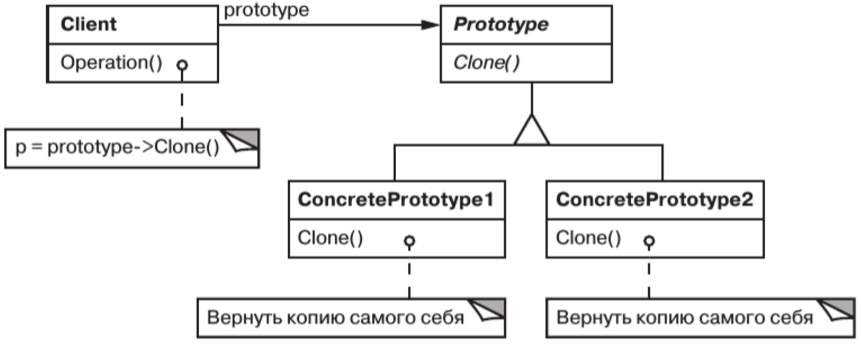
\includegraphics[width=0.85\textwidth]{prototype.png}
        \end{center}
    \end{frame}
    
    \begin{frame}
        \frametitle{``Прототип'', детали реализации}
        \begin{itemize}
            \item Можно реализовать через рефлексию (но не нужно)
            \item Реестр прототипов, обычно ассоциативное хранилище
            \item Операция Clone
            \begin{itemize}
                \item Глубокое и мелкое копирование
                \item В случае, если могут быть круговые ссылки
                \item Сериализовать/десериализовать объект (но помнить про идентичность)
            \end{itemize}
            \item Инициализация клона
            \begin{itemize}
                \item Передавать параметры в Clone --- плохая идея
            \end{itemize}
        \end{itemize}
    \end{frame}

\end{document}
